\chapter{Resultater} \label{title:resultater}


\section{Konditioneringsapparat}
Konditioneringsapparatet er opbygget af flere blokke, som kan ses på figur \ref{fig:BDD(SystemOverview)}. Blok Definition diagrammer beskriver relationerne mellem blokke, så som sammenhæng, forening og specialisering. I denne sammenhæng beskriver figur \ref{fig:BDD(SystemOverview)} opbygningen af konditioneringsapparatet. 
\begin{figure}[H]
	\centering
	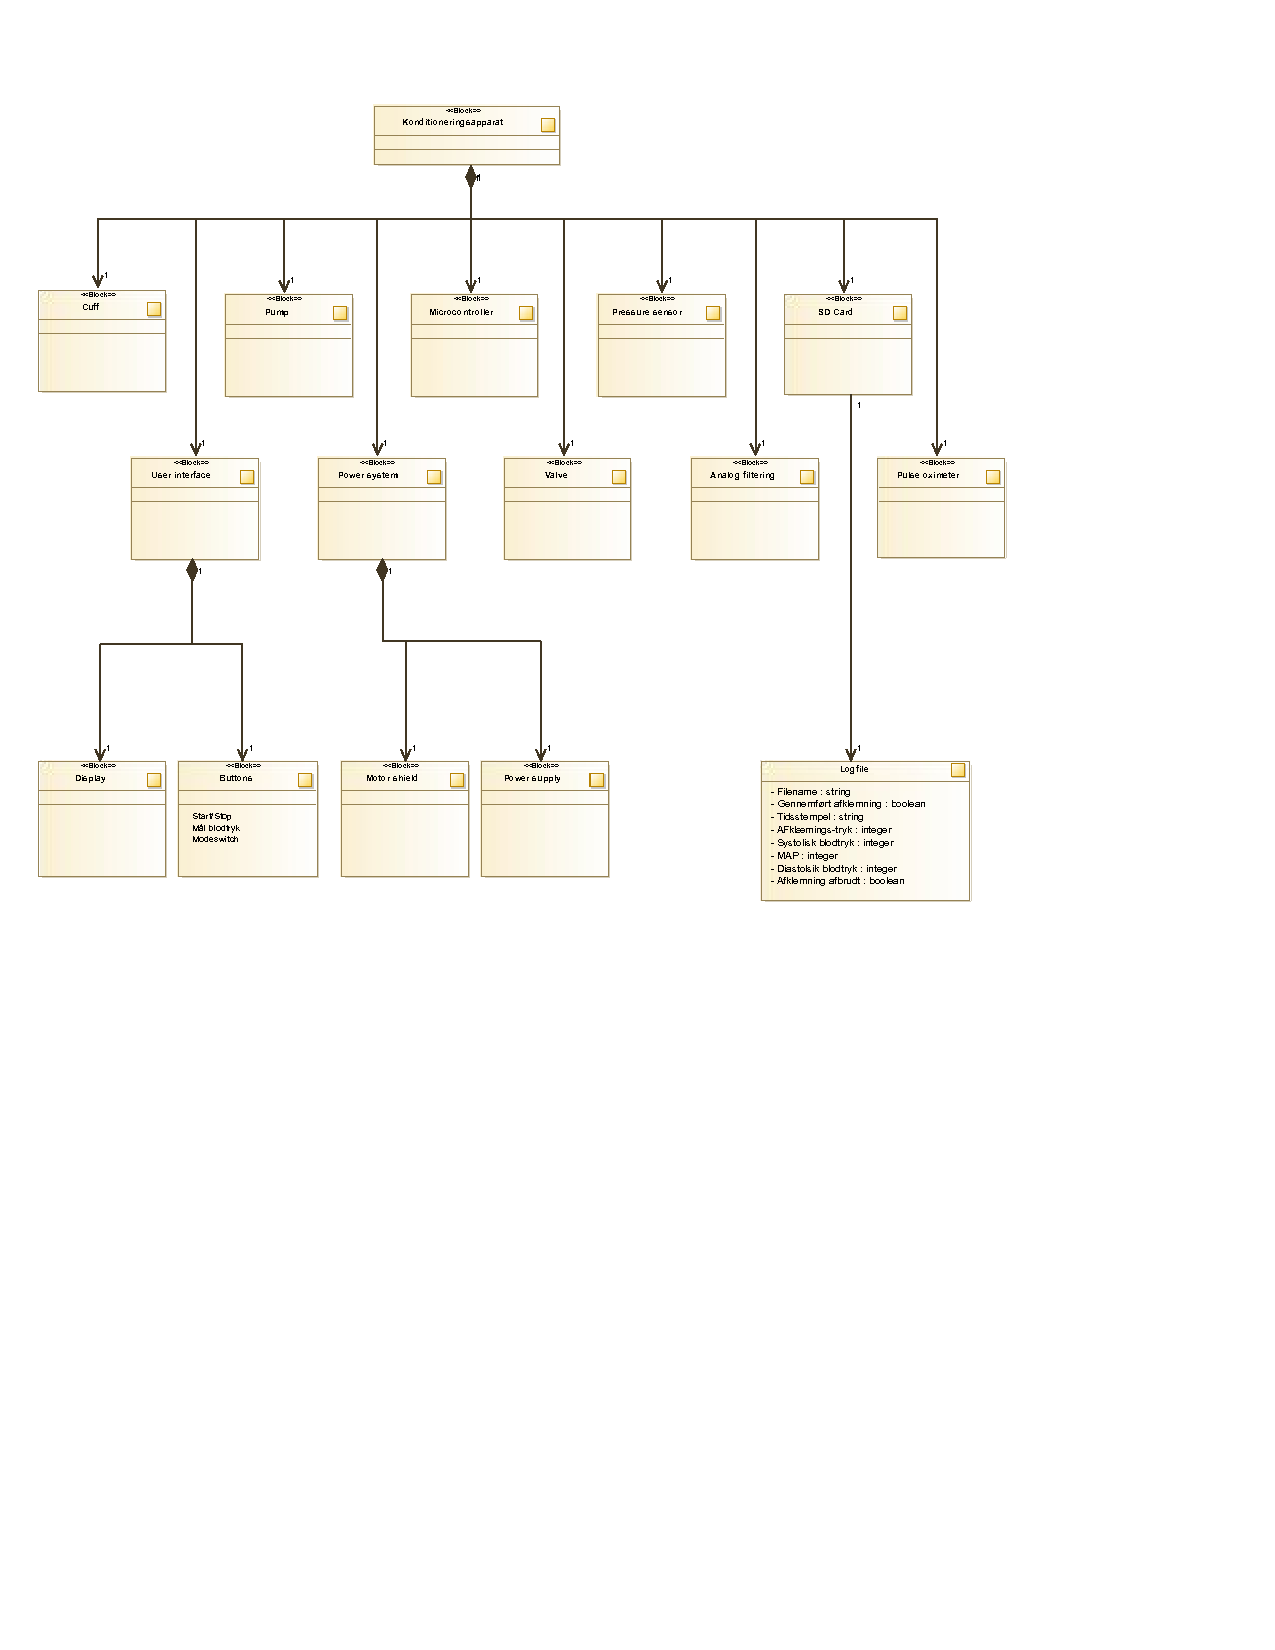
\includegraphics[width=0.9\textwidth]{billeder/BDD(SystemOverview).pdf}
	\caption{Block difinition diagram over konditioneringsapparatet.}\label{fig:BDD(SystemOverview)}
\end{figure}

\subsection{Oscilumetrisk blodtryks apparat}
Den oscillometriske blodtryks måle metode, beskrevet i afsnit \ref{noninvasivBloodpressureMeasurement}, er implementeret i implementeringsdokumentet\fixme{reff: implementeringsdokument} og resultaterne er beskrevet i dette afsnit.

Det pulserende signal fra tryksensoren, som blodtryksmåleren analyserer er i sin rå (ubehandlet) tilstand støjfyldt. Signalet beskrevet i afsnit \ref{noninvasivBloodpressureMeasurement} på figur \ref{fig:OscillometriskMetode} er meget rent og amplitudehøjderne danner en flot parabel formet kurve. På figur \ref{fig:rawPulseSignal} ses det pulserende signal direkte fra tryksensoren, som er indhyldet i støj. Kurven er stødt faldende, fordi trykket i manchetten langsomt lukkes ud. Ydermere observeres der også varierende amplitudehøjder, som ikke er stødt stigende/faldende, men virker som tilfældigheder.  

\begin{figure}[H]
	\centering
	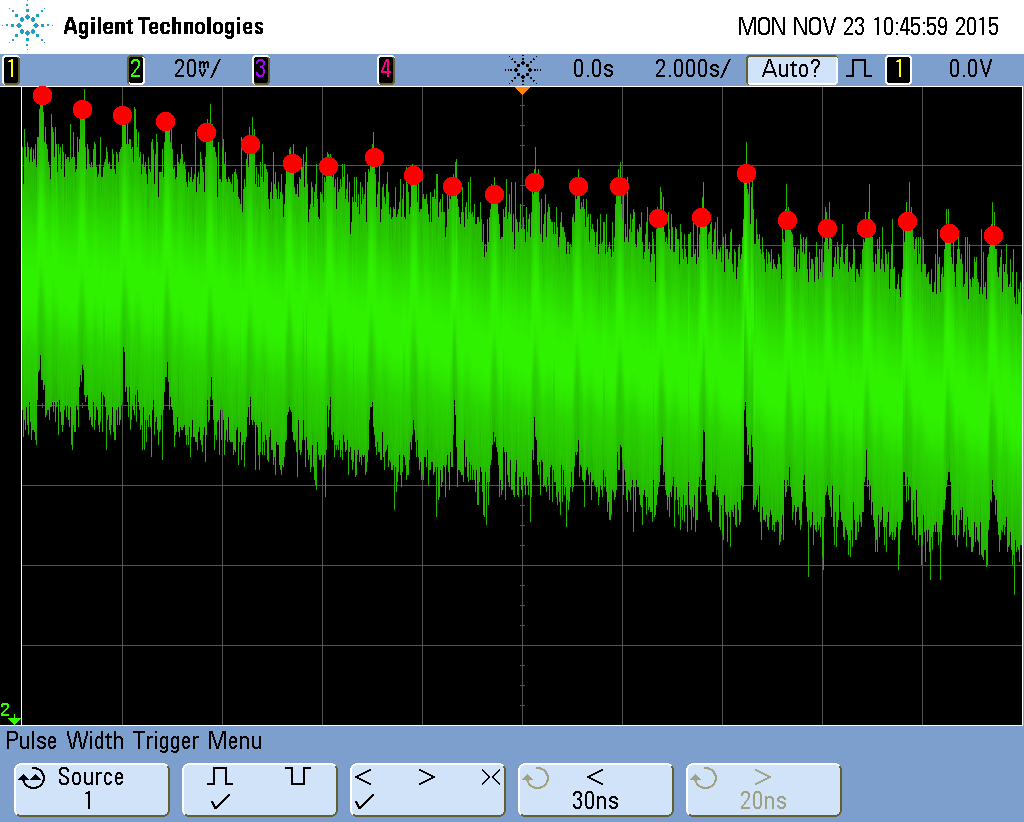
\includegraphics[trim={0 7cm 0 1.5cm},clip, width=1\textwidth]{billeder/rawPulseSignalPeaks.png}
	\caption{Oscilloskops måling af rå signal fra blodtryksmåling, med konditioneringsapparatet. De røde cirkler er pulse oscillationernes højeste punkt}\label{fig:rawPulseSignal}
\end{figure}

Efter analog filtrering af det rå signal på endnu en blodtryksmåling med konditioneringsapparatet, ses at amplitude oscillationerne isoleret og uden manchettrykket (offset). Over en hel blodtryksmåling skal kurven ifølge teorien (se figur \ref{fig:OscillometriskMetode}), starte med en stigende amplitude højde efterfulgt af en top og til sidst faldende oscillationshøjder med laverer hældnings koefficient end starten. En hel blodtryksmåling med filtreret råsignal kan ses på figur \ref{fig:filteredPulseSignal}.

\begin{figure}[H]
	\centering
	\subbottom[Stigende]{%
		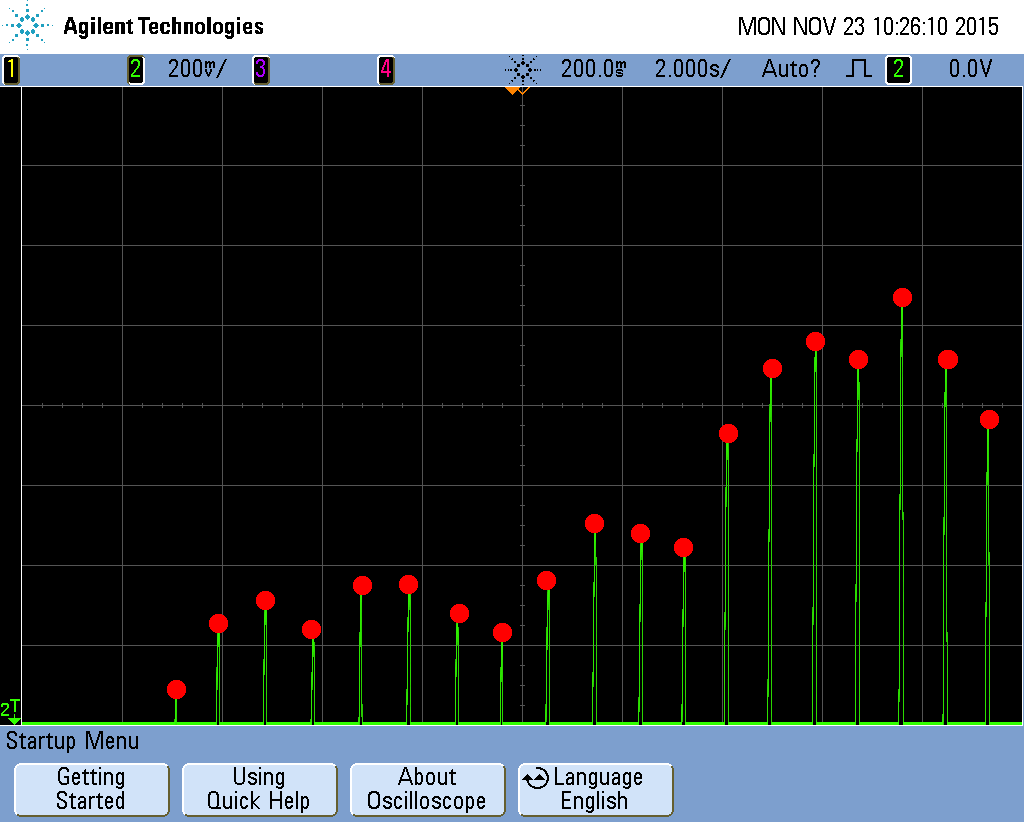
\includegraphics[trim={0 3.3cm 0 1.5cm},clip, width=0.328\textwidth]{billeder/filteredPulseSignalPeaks1.png}}
	\subbottom[Højdepunkt]{%
		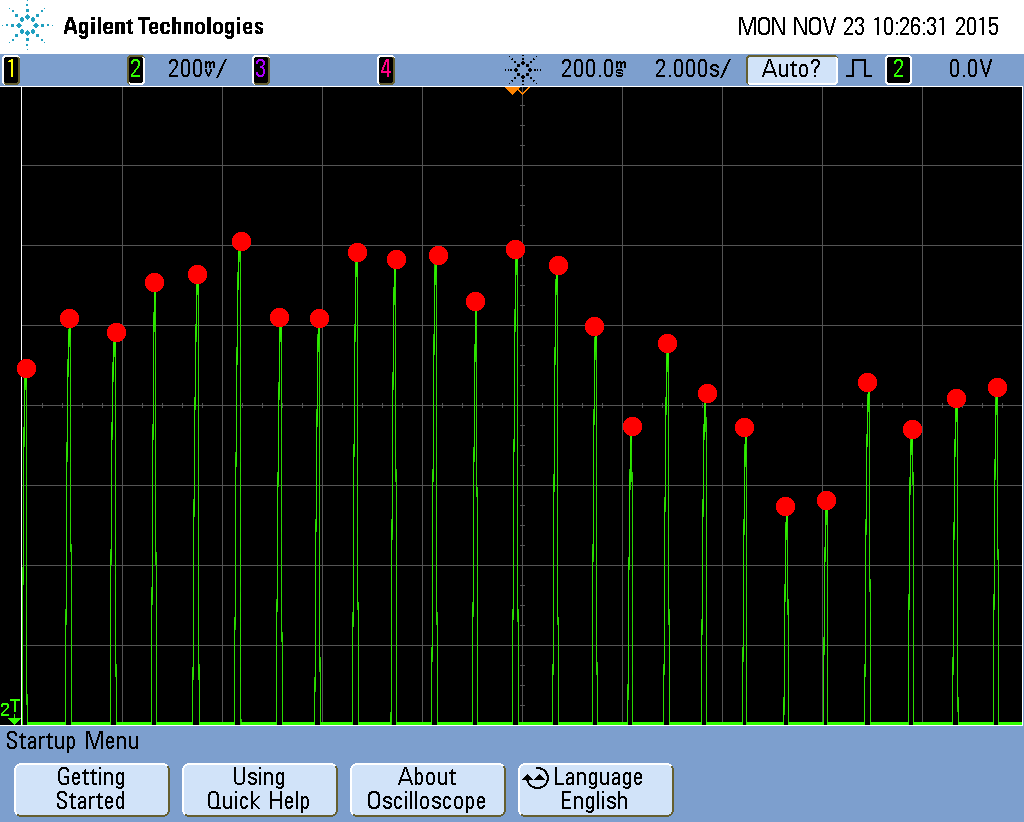
\includegraphics[trim={0 3.3cm 0 1.5cm},clip, width=0.328\textwidth]{billeder/filteredPulseSignalPeaks2.png}}
	\subbottom[Faldende]{%
		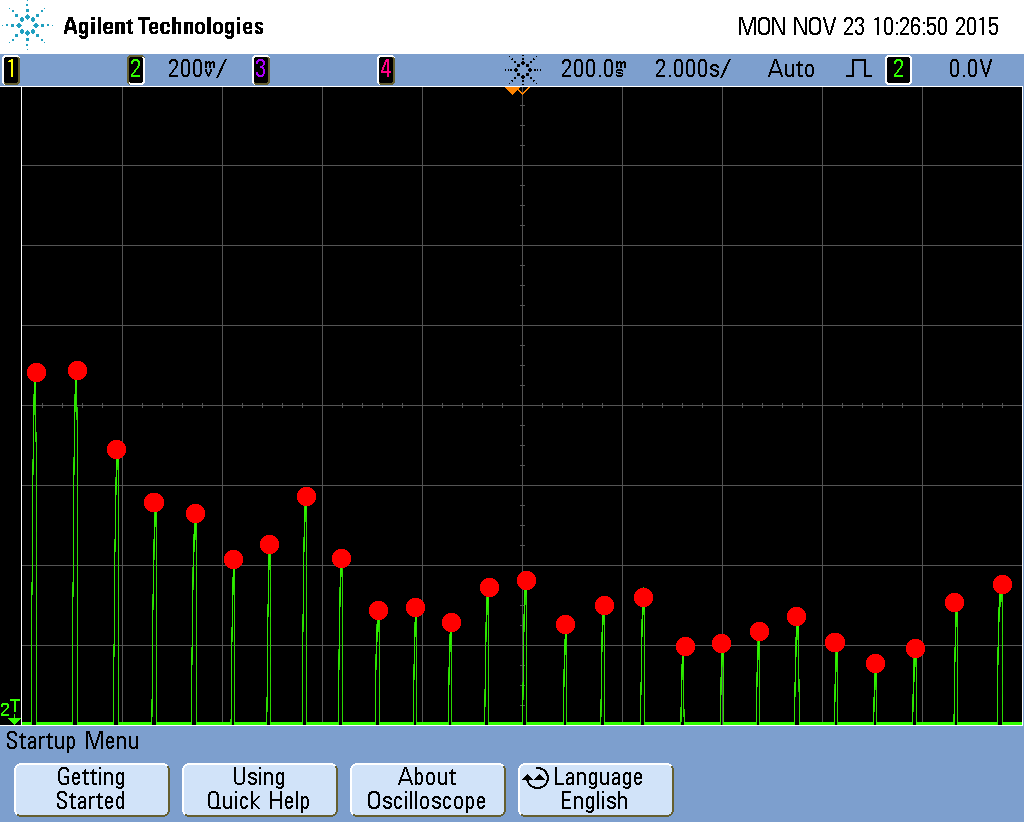
\includegraphics[trim={0 3.3cm 0 1.5cm},clip, width=0.328\textwidth]{billeder/filteredPulseSignalPeaks3.png}}
	\caption{Osclilloskops måling af filtreret signal af blodtryksmåling, med konditioneringsapparatet. (a) er første del af blodtryksmålingen, (b) er de midten af signalet med, hvor MAP befinder sig og (c) er slutningen af signalet, hvor amplituderne flader ud. De røde cirkler er pulse oscillotionernes højeste punkt}\label{fig:filteredPulseSignal}
\end{figure}

\subsubsection{Analog filtrering}
Den analoge filtrering, ses på forskellen mellem figur \ref{fig:rawPulseSignal} og figur \ref{fig:filteredPulseSignal}, er implementeret i implementeringsdokumentet se \fixme{ref: implementeringsdokument}. 
Det resulterende analoge filter, er bestemt ud fra test opsætninger (se \fixme{ref: implementeringsdokument}) og litteraturen \fixme{CHARACTERIZATION OF THE OSClLLOMETRlC METHOD FOR MEASURING INDIRECT BLOOD PRESSURE}. De pulserende oscillationer isoleret fra det rå signal kan ses på figur \ref{fig:filteredPulseSignalWithFFT}. Resultatet er opnået, ved at implementere et båndpasfilter, med et pasbånd som starter før lavest mulige puls\fixme{fortæl hvad det er} og slutter ved den tiende afledte af grundfrekvensen 60bmp (se figur \ref*{fig:BandPassFilter}).

\begin{figure}[H]
	\centering
	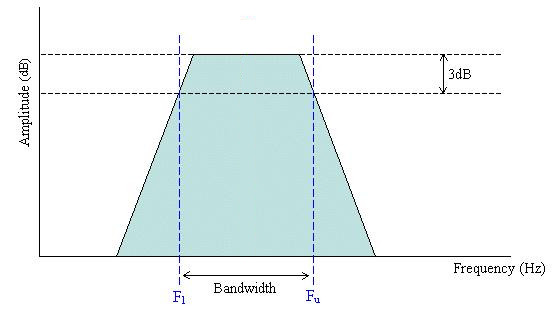
\includegraphics[trim={0 0 0 1.5cm},clip, width=0.8\textwidth]{billeder/BandPass_filter.JPG}
	\caption{Bånd pass filter med passfilter mellem $F_1$ og $F_u$. $F_1=0.22Hz$ (13 bmp under mulig puls) og $F_u=11Hz$ (660 bmp 10 afledte af 60 bpm) }\label{fig:BandPassFilter}
\end{figure}

\begin{figure}[H]
	\centering
	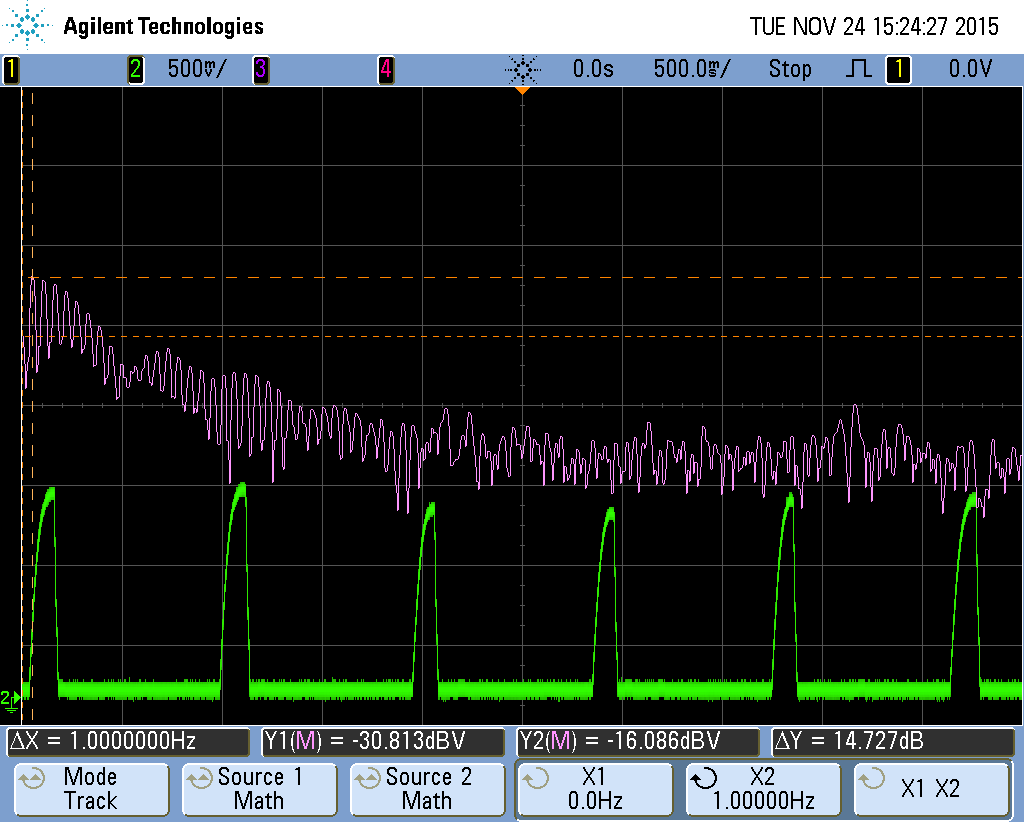
\includegraphics[trim={0 2.5cm 0 1.5cm},clip, width=0.8\textwidth]{billeder/filteredPulseSignalWithFFT.png}
	\caption{Osclilloskops måling af filtreret signal fra manchetten oppustet på arm. Den grønne kurve er de pulserende oscillotioner og den lilla kurve er en Fast Fourier Transformation (FFT) af den grønne kurve, hvor den udregnede grundfrekvens af oscillationerne måles til 1Hz (60 bpm).}\label{fig:filteredPulseSignalWithFFT}
\end{figure}

\subsubsection{Digital filtrering}
For at opnå en glat parabel, som vist på  figur \ref{fig:OscillometriskMetode}, er der implementeret et digitalt filter, som har til opgave at udglatte oscillutions amplituderne fra blodtryksmålingerne. Resultatet af implementeringen kan ses på figur \ref{fig:digitalFilterData}. Det bedste forhold mellem udglatning og reaktionshastighed af filteret er opnået ved et ekspotentielt midlingsfilter (se \ref{eq:ekspotentielmidlingsfilter}) med alfa værdi på 0.15 (se \fixme{reff: implementeringsdokument} for uddybende beskrivelse).  

\begin{equation}
y(n)=\alpha*x(n)+(1-\alpha)*y(n-1)
\label{eq:ekspotentielmidlingsfilter}
\end{equation}
\begin{figure}[H]
	\centering
	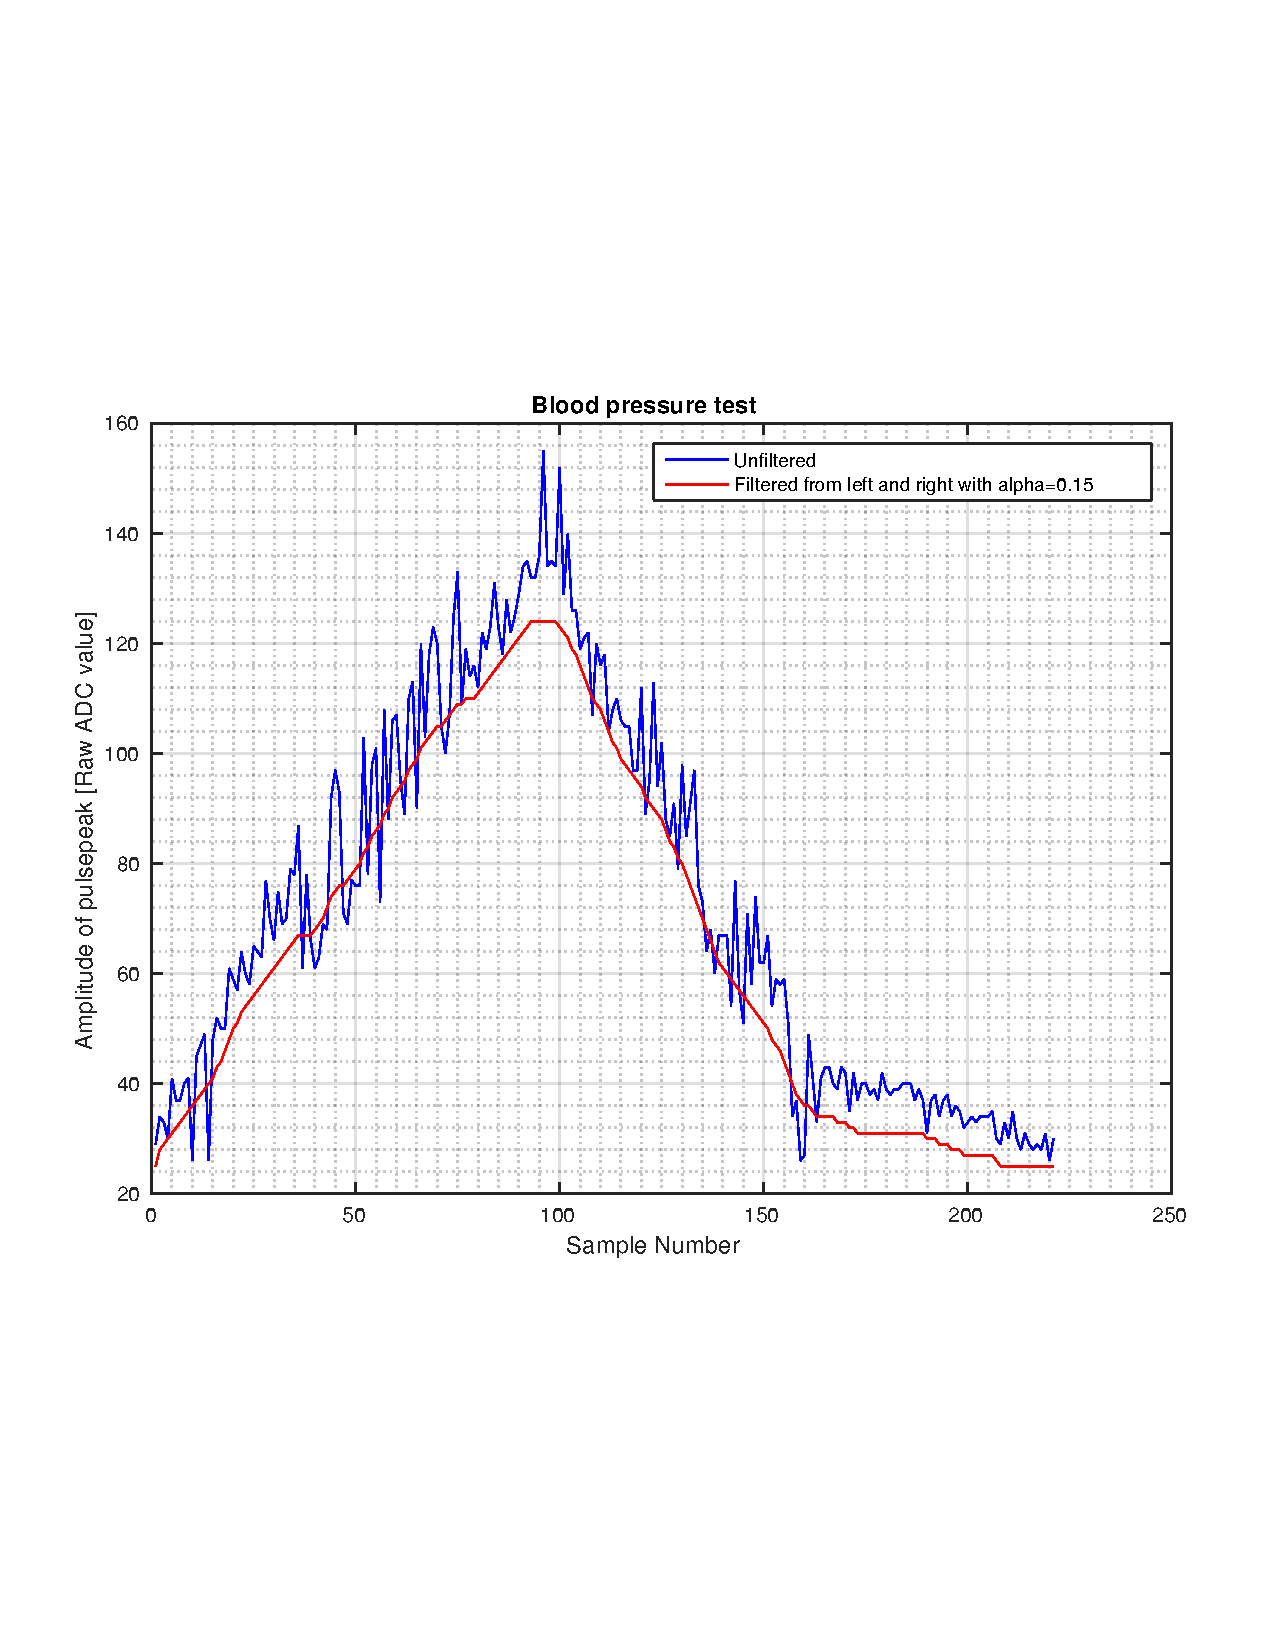
\includegraphics[trim={0 0 0 0},clip, width=0.7\textwidth]{billeder/digitalFilterData.pdf}	
	\parbox{10.5cm}{\caption{Digital filtrering af oscillotions peaks fra blodtryksmåling på simulator med ekspotentiel midlingsfilter.}\label{fig:digitalFilterData}}
\end{figure}


\subsection{Fikseret-ratio} \label{Fikseret-ratio}
Konditioneringsapparatets mest avancerede egenskab er uden tvivl estimering af blodtrykket. Apparatet anvender den oscillometriske metode hvor det systoliske og diastoliske tryk blandt andet bestemmes ud fra MAP. Under udviklingen af konditioneringsapparatet blev det besluttet at anvende den fikserede-ratio metode for at forsimple udviklingsarbejdet.

Fikseret-ratio metoden anvender empirisk data til at bestemme hvor store oscillationerne i manchettenv skal være i forhold til oscillationerne ved MAP, for at identificerer SYS og DIA. Dette betyder at systolisk og diastolisk tryk er bestemt ved manchettrykket når amplituden af oscillationerne er en ratio af den maksimale værdi.\fixme{ref: Theory of the Oscillometric Maximum and the Systolic and Diastolic Detection Ratios}

\begin{minipage}[c]{0.5\textwidth}
	Ratio værdierne til \textit{konditioneringsapparatet} kunne ikke bestemmes ud fra en større mængde empirisk data fra patienter, på grund af projektets omfang. I stedet er empirisk data blevet indsamlet fra "Fluke biomedicalBP Pump 2" en oscillometrisk blodtrykssimulator (se figur \ref{fig:TheFlukeBiomedicalBPPump2L}). \textit{Konditioneringsapparatet} opsamlede data fra simulatoren, hvilket kan ses på figur \ref{fig:digitalFilterData} og \ref{fig:digitalFilterDataSysMapDia}. Fordi simulatoren indstilles til kendte blodtryksværdier kan de fikserede-ratiorer bestemmes ud fra oscillations amplituden (OA) ved et givent manchettryk. f.eks ved simulering af 120/80 skal oscillations amplituden ved manchettrykket 120mmHg aflæses og forholdet mellem MAP og denne aflæste værdi er den systoliske ratio.
	
	
\end{minipage}
\begin{minipage}[c]{0.5\textwidth}
	\begin{figure}[H]
		\centering
		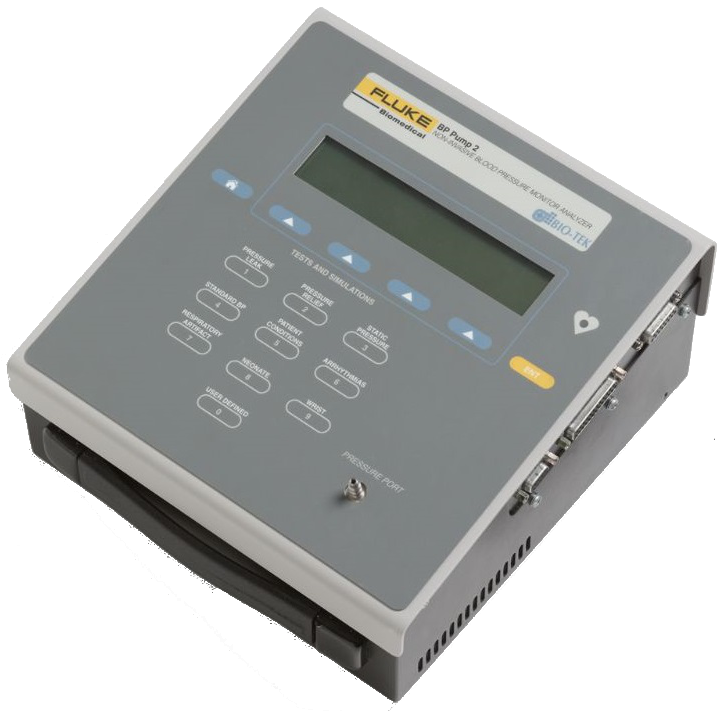
\includegraphics[trim={0 0 0 0},clip, width=0.9\textwidth]{billeder/TheFlukeBiomedicalBPPump2L.png}	
		\parbox{7cm}{\caption{Fluke Biomedical BP Pump 2 Non-invasiv blodtrykssimulator}\label{fig:TheFlukeBiomedicalBPPump2L}}
	\end{figure}
\end{minipage}

Resultatet af simulationerne kan ses på figur \ref{fig:digitalFilterDataSysMapDia1} uden manchettrykket og med manchettrykket på figur \ref{fig:digitalFilterDataSysMapDia2}. Ratioen for SYS (se \ref{eq:sysratio}) blev udregnet til 0.38 og for DIA (se \ref{eq:sysratio}) til 0.48. 
	\begin{equation}
	SYS_{OA}=MAP_{OA}*0.38
	\label{eq:sysratio}
	\end{equation}
	\begin{equation}
	DIA_{OA}=MAP_{OA}*0.48
	\label{eq:diaratio}
	\end{equation}

\begin{figure}[H]
	\centering
	\subbottom[Simulationsdata uden manchettryk]{\label{fig:digitalFilterDataSysMapDia1}%
		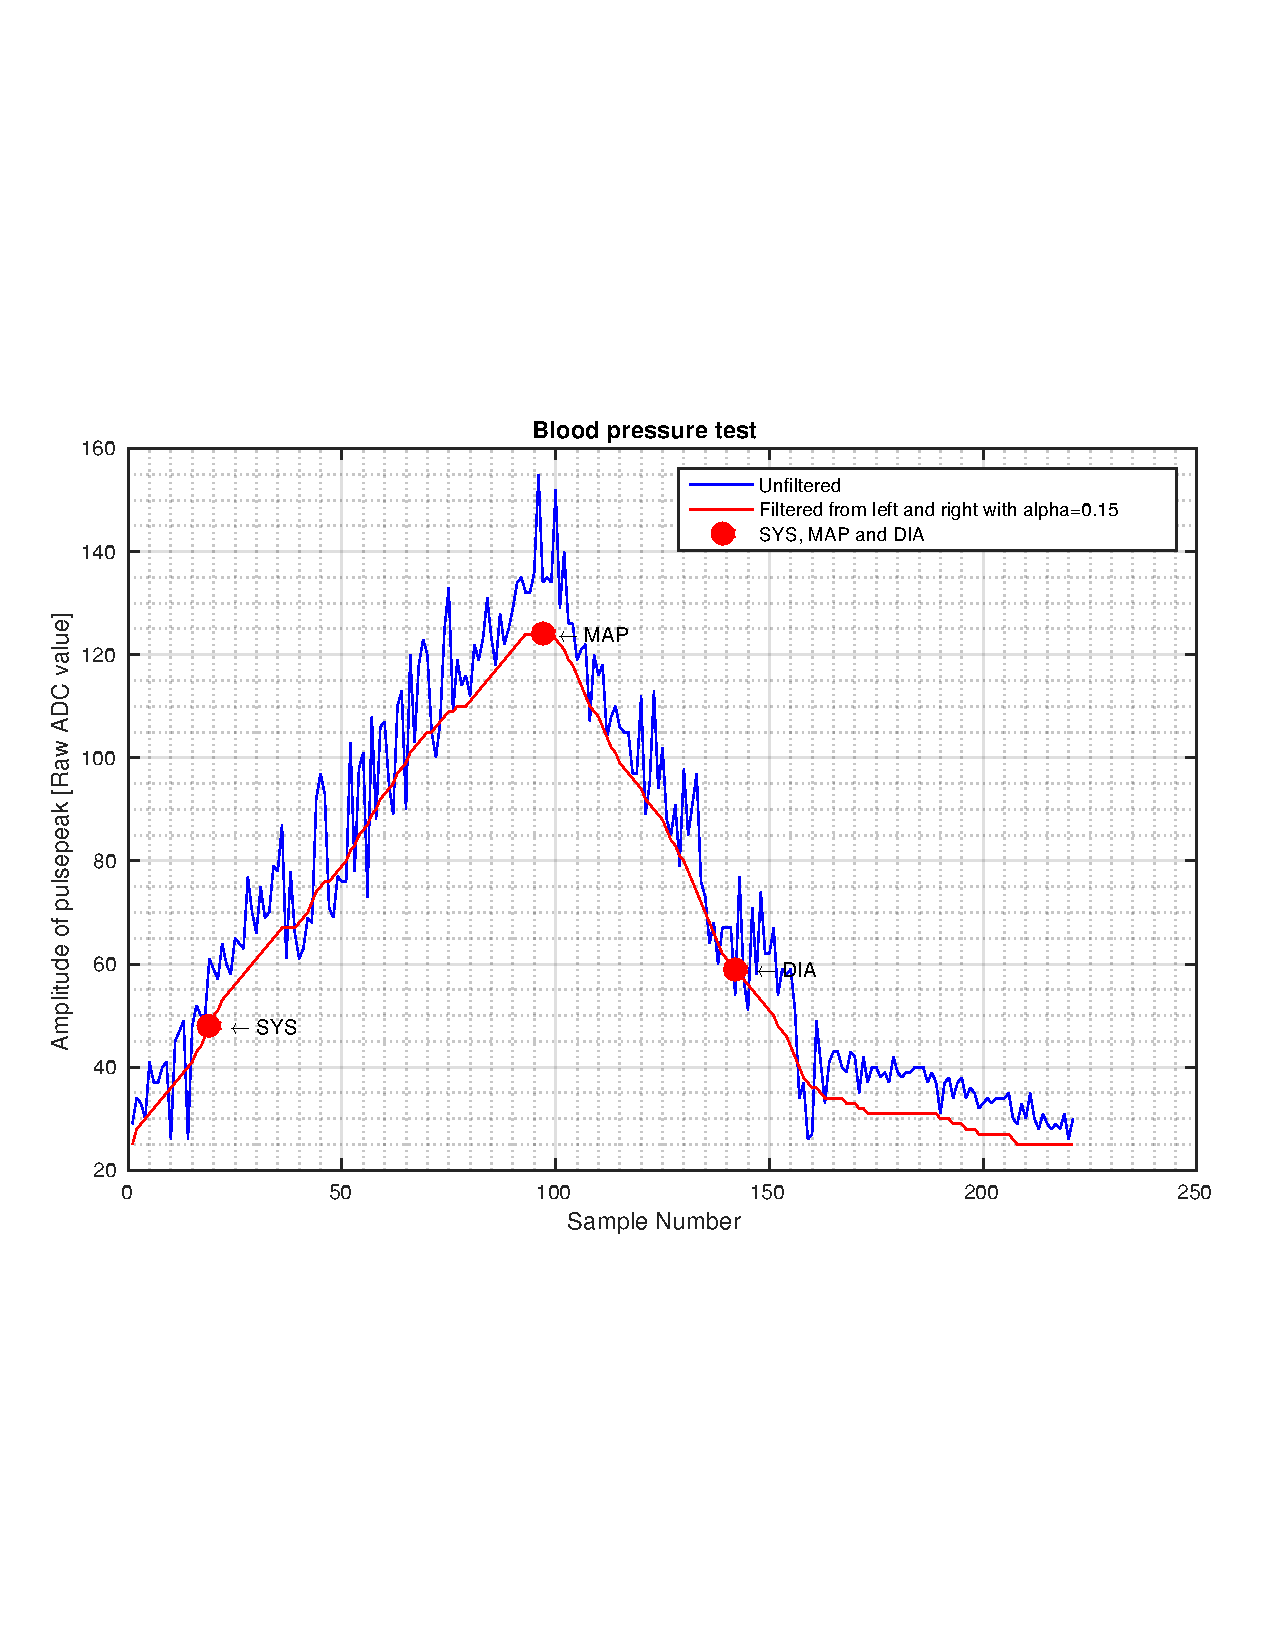
\includegraphics[trim={0 0 0 0},clip, width=0.48\textwidth]{billeder/digitalFilterDataSysMapDia.pdf}}
	\subbottom[Simulationsdata med manchettryk]{\label{fig:digitalFilterDataSysMapDia2}%
		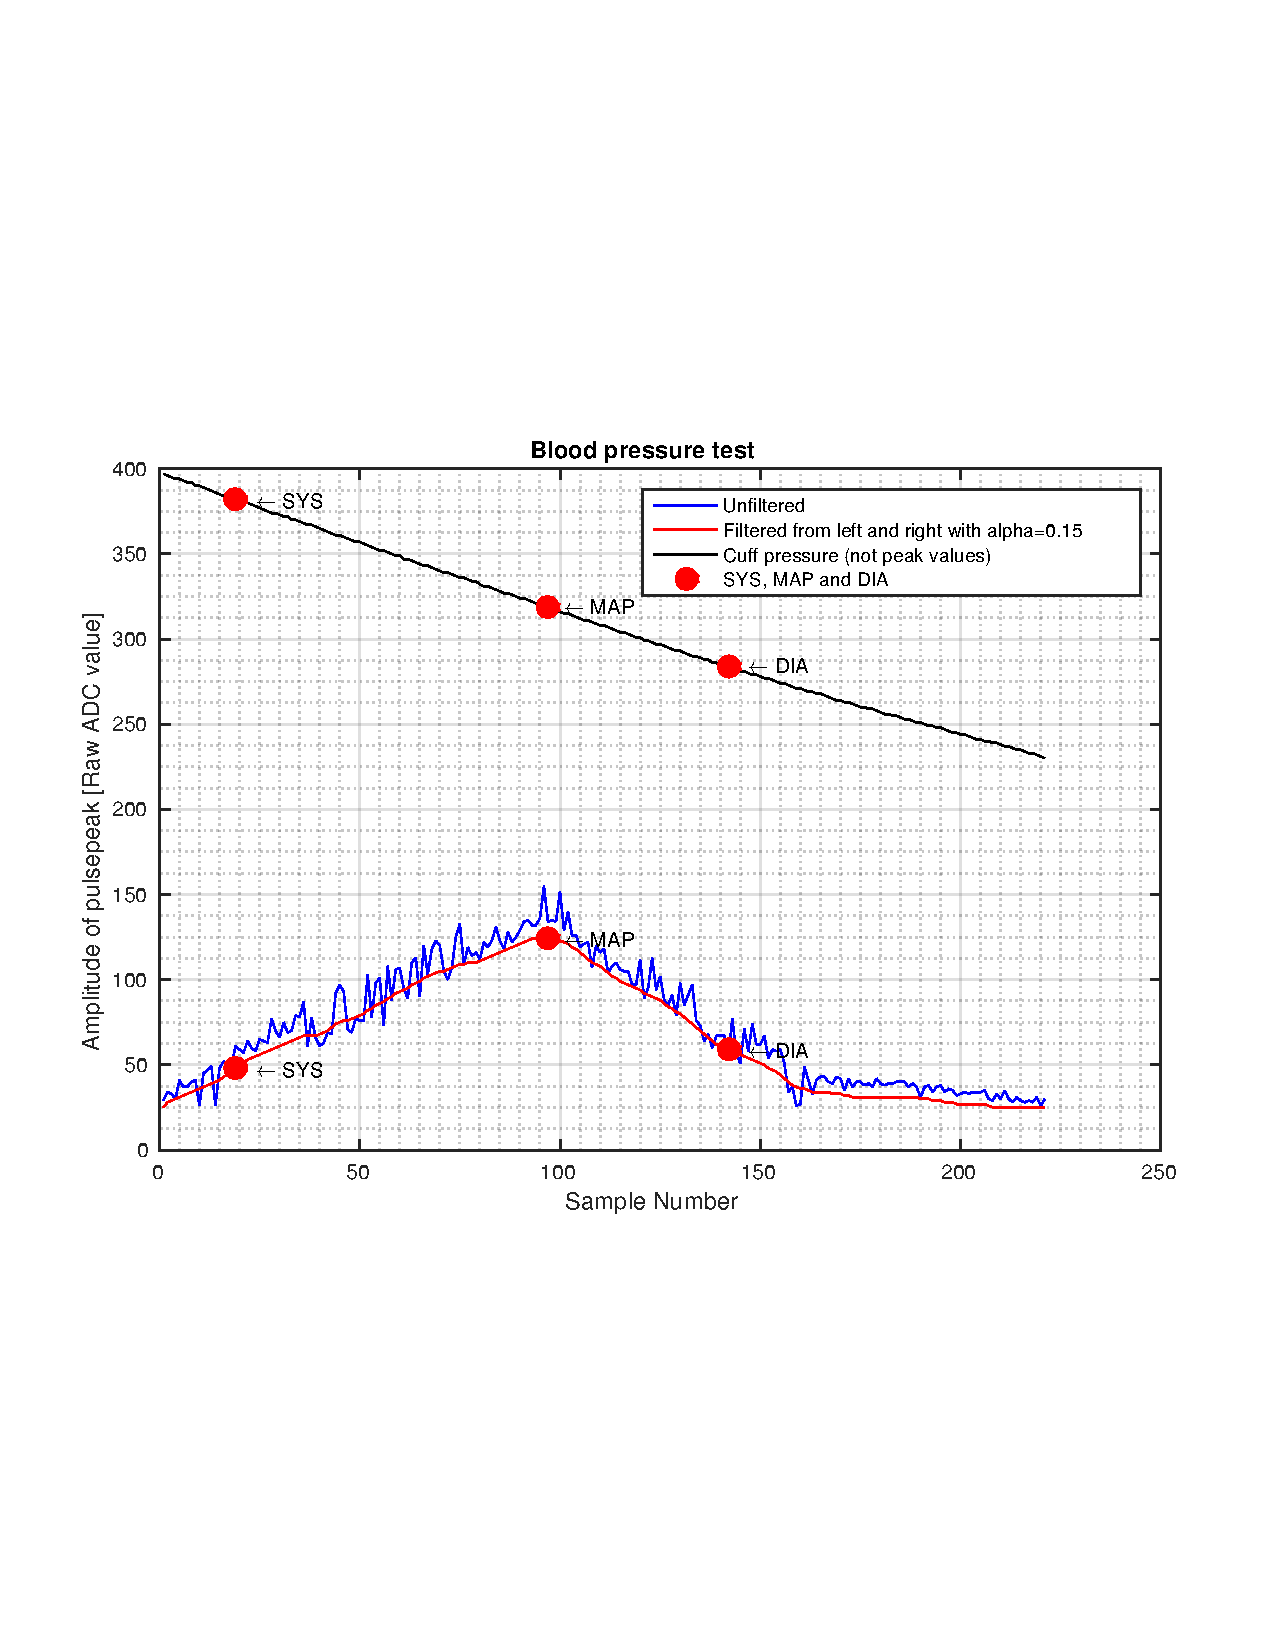
\includegraphics[trim={0 0 0 0},clip, width=0.48\textwidth]{billeder/digitalFilterDataCuffSysMapDia.pdf}}
	\caption{Digital filtrering af oscillotions amplituderne fra blodtryksmåling på simulator med ekspotentiel midlingsfilter. De røde prikker er placeret  hvor SYS, MAP og DIA befinder sig ved fikseret-ratio på 0.38(SYS) og 0.48(DIA).}
\end{figure}
  

\subsection{Dataopsamling}
I forbindelse med udviklingen af prototypen var der et ønske fra kunden side omkring dataopsamling fra \textit{Konditioneringsapparatet}. For at apparatet kan bruges til forskningsprojektet er nødvendigt, at kunne dokumentere hvor mange konditioneringscyklusser en patient har modtaget. I samarbejde med kunden blev aftalt at et \textit{konditioneringsapparat} skal følge en patient i gennem hele forløbet, altså fra præhospital, til hospital og til sidst i hjemmet. Derfor blev det besluttet at data blev gemt på et SD kort, som hver gang et apparat returneres fra en patient bliver tømt for data og formateret. 

\begin{figure}[H]
	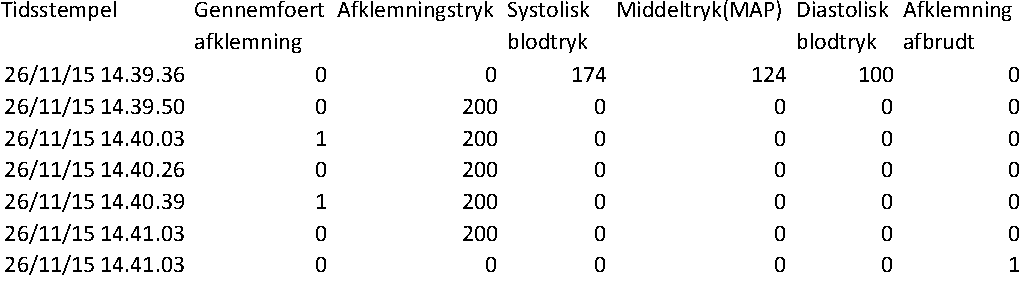
\includegraphics[width = \textwidth]{billeder/fileksempel-crop.pdf}
	\caption{Et eksempel på fil udtræk fra SD kortet}\label{fig:fileksempel}
\end{figure}

På figur \ref{fig:fileksempel} oversigt over fil udtræk. Her er udført en konditioneringsbehandling, hvor blodtrykket først er blevet målt til 174/100(124) mmHg. Der gemmes en værdi ved blodtryksmåling, hver gang trykket i manchetten når afklemningstrykket og når en okklusionsfase er færdig. Endvidere skrives det til SD kortet hvis konditioneringsbehandlingen afbrydes. Hver gang der skrives til SD kortet gemmes et tidsstempel, om afklemningen er gennemført, afklemningstrykket, blodtrykket og information omkring konditioneringsbehandling blev færdig gjort. 

I den måling der er vist på figur \ref{fig:fileksempel} er der foretaget en blodtrykmåling, 2 fulde cyklusser og en afbrudt cyklus. En okklusion cyklus var sat til 10 sekunder og antallet af cyklusser var 3. Grundet til tidsstemplerne ikke er med 10 sekunder forskel er at der først skrives til SD kortet når afklemningstrykket er højere end det målte systoliske tryk.. Det tager lidt tid for motoren at pumpe manchetten op til dette tryk. 

For at sikre at informationen på SD kan kobles til en patient, genereres der et unikt ID på 5 hexidecimaler, som sammen med apparat ID'et på 3 cifre, bliver til navnet på filen. Filen der er vist på figur \ref{fig:fileksempel} har derfor navnet \textit{93C09001.csv}. \textit{93C090} er det unikke patient ID og \textit{001} er apparat ID. Når den første måling fortages på et apparat med formateret SD kort bliver der generet en .csv fil med det 8 cifrede navn. Patient ID bliver vist på skærmen af \textit{Konditioneringsapparatet}. Patient ID'et skal noteres at ambulance personalet, Patient ID'et parres med CPR nummeret, så dette er utilgængeligt for alle involveret i forskningsprojektet. Dette gøres for at apparatet ikke skal håndtere patient følsomme oplysninger.

\subsection{Pulsoximetri} \label{title:pulsOxi}
Som beskrevet i projektafgrænsninger (se afsnit \ref{title:sikkerhedskontrol}) blev projektet afgrænset fra at have sikkerhedskontrol med pulsoximeteri. For at bekræfte pulsoximeteri var et brugbart til sikkerhedskontrol, har projektgruppen foretaget test med pulsoximeter. Formålet med testen var at se om puls og saturation gav nogle brugbare udsving efter en endt okklusionsfase. I testen blev der lavet to fulde cyklusser, hver især bestod af en 5 minutters okklusionsfase efterfulgt af en 5 minutters reperfusionsfasen. Saturation og puls var de målbare parametre i denne test. Parametrene blev noteret lige før okklusionsfasen blev påbegyndt, hvert 30. sekunder under okklusionen og hhv. 10, 20 og 30 sekunder inde i reperfusionsfasen. Pulsoximeteret der blev brugt til målingerne var fra EDAN, model H100B (Se datablad \cite{RefWorks:30}). Blodtrykket på testpersonen var målt til 120/63 mmHg og afklemningstrykket blev valgt til 220mmHg. Trykket i manchetten lå med en tolerance på +/-20 mmHg under okklusionsfasen. 

Testen viste ingen indikation af udsving i saturationen når armen var afklemt. Når trykket i manchetten faldt, fandt pulsoximeter med det samme puls og saturation. Pulsen der blev fundet, lå på samme niveau før og efter okklusionsfasen. Saturation var i begge tilfælde cirka 20 sekunder om at nå tilbage til samme værdi, som før okklusionsfasen. \fixme{Reference til test resultatet}

\subsection{Konditionering}
\textit{Konditioneringsapparatets} hovedfunktion er, som beskrevet i problemformuleringen (afsnit \ref{title:problemformulering}), konditionering af patienter deltagende i RIC forskningsstudiet (afsnit \ref{title:studieprotokold}). Resultaterne af konditioneringsbehandlingens implementering i apparatet er som beskrevet i resultater af accepttesten (se afsnit \ref{title:accepttest}) gode. \textit{Konditioneringsapparatet} kan foretage en non-invasiv blodtryksmåling, med den ocillometriske fikseret-ratio metode. Ud fra det målte blodtryk foretager apparatet en okklusion med et tryk på 25mmHg over systolisk tryk, dog med et minimumstryk på 200mmHg og et maksimumstryk på 300mmHg. Okklusionsfasen varer et tidsrum predefineret af brugeren. Okklusionsfasen efterfølges af en reperfusionsfase, som tidsmæssigt er tilsvarende okklusionsfasen. Ved gennemførsel af de to faser tæller \textit{Konditioneringsapparatet} antal cykluser tilbage, en ned. Den totale mængde af cykluser, som skal gennemføres for en konditionering er prædefineret af brugeren.

\subsection{Okklusionstræning}
Resultatet af okklusionstræningen, er et apparat, som holdet et konstant tryk i manchetten, alt imens et kører et stopur på skærmen. Trykket i manchetten fyldes til 100mmHg. Trykket falder herefter stille og roligt til under 90mmHg hvorefter trykket i manchetten igen opreguleres til 100mmHg ved hjælp af pumpen. 
 
\subsection{Grafisk interface}
Det blev specificeret i kravspecifikationen at \textit{Konditioneringsapparatet} skulle levere feedback til bruger ved hjælp af et display (Se kravspecifikationen\fixme{Reference til kravspecifikation}). Resultatet af dette krav, blev implementering af et 2.2" farve display. Af de forskellige brugerfeedbacks displayet leverer, er det værd at fremhæve manchettrykket, patient ID, antal cyklusser og tidsforløbet. Visningen af manchettrykket er vigtigt, for at brugeren eller medicinsk personale kan observere at konditioneringsbehandling er i gang med okklusion eller reprefusion. Tidsinformation omkring konditioneringsbehandling sikre at patienten og medicinsk personale kender til den resterende tid af behandlingen. I tilfælde hvor patienten skal modtage anden behandling eller kontrol hvor \textit{Konditioneringsapparatet} ikke kan være monteret, kan tidsinformation hjælpe med beslutningen om hvornår apparatet skal afmonteres. 

\begin{figure}[H]
\centering
\subbottom[Konditioneringsforløb]{%
	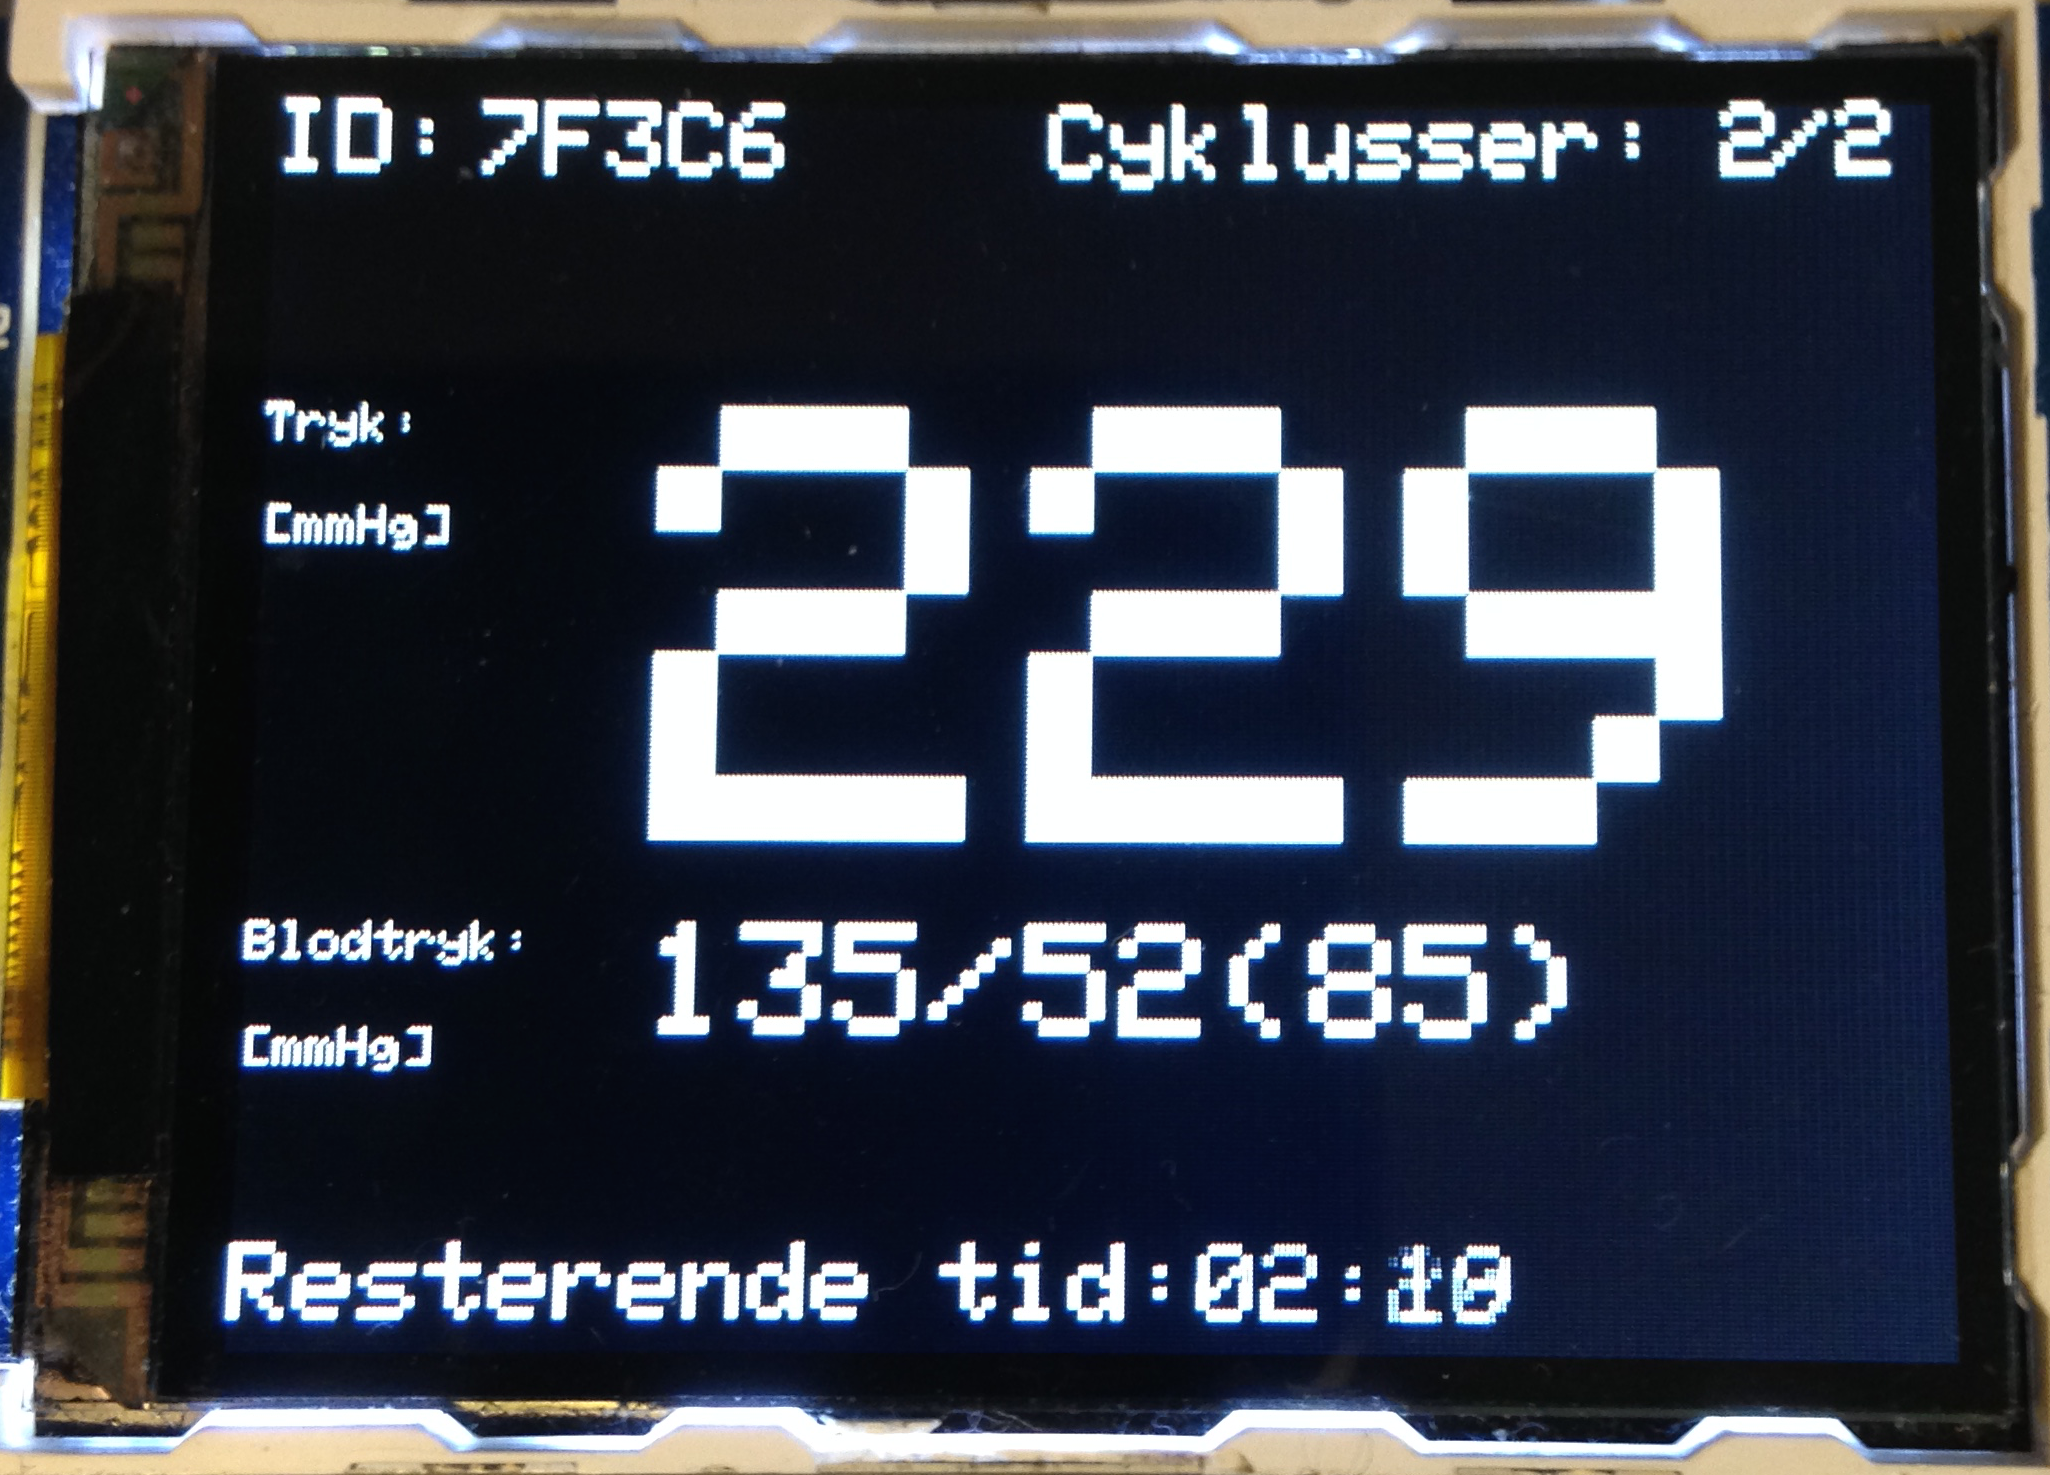
\includegraphics[trim={0 3.3cm 0 1.5cm},clip, width=0.328\textwidth]{billeder/display/konditionering.png}}
\subbottom[Okklusionstræning]{%
	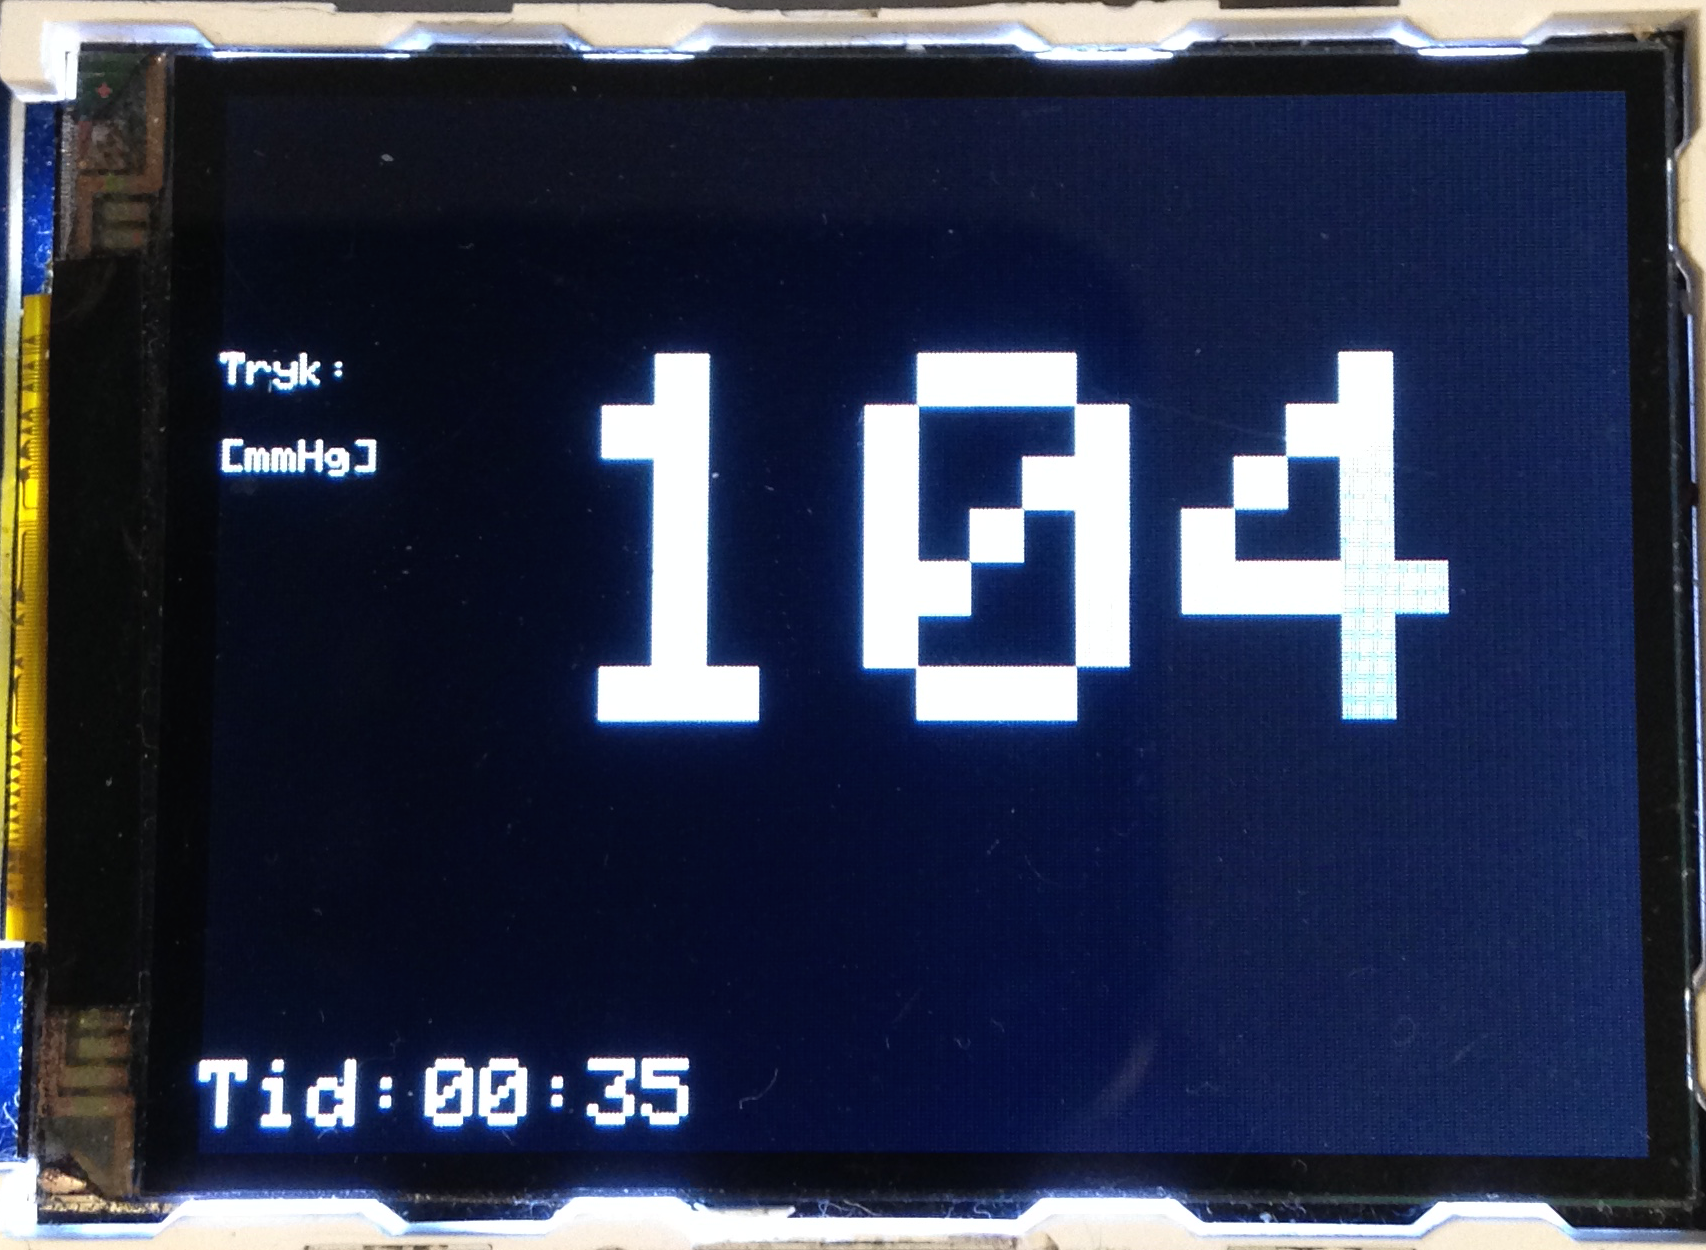
\includegraphics[trim={0 3.3cm 0 1.5cm},clip, width=0.328\textwidth]{billeder/display/okklusion.png}}
\subbottom[Setup]{%
	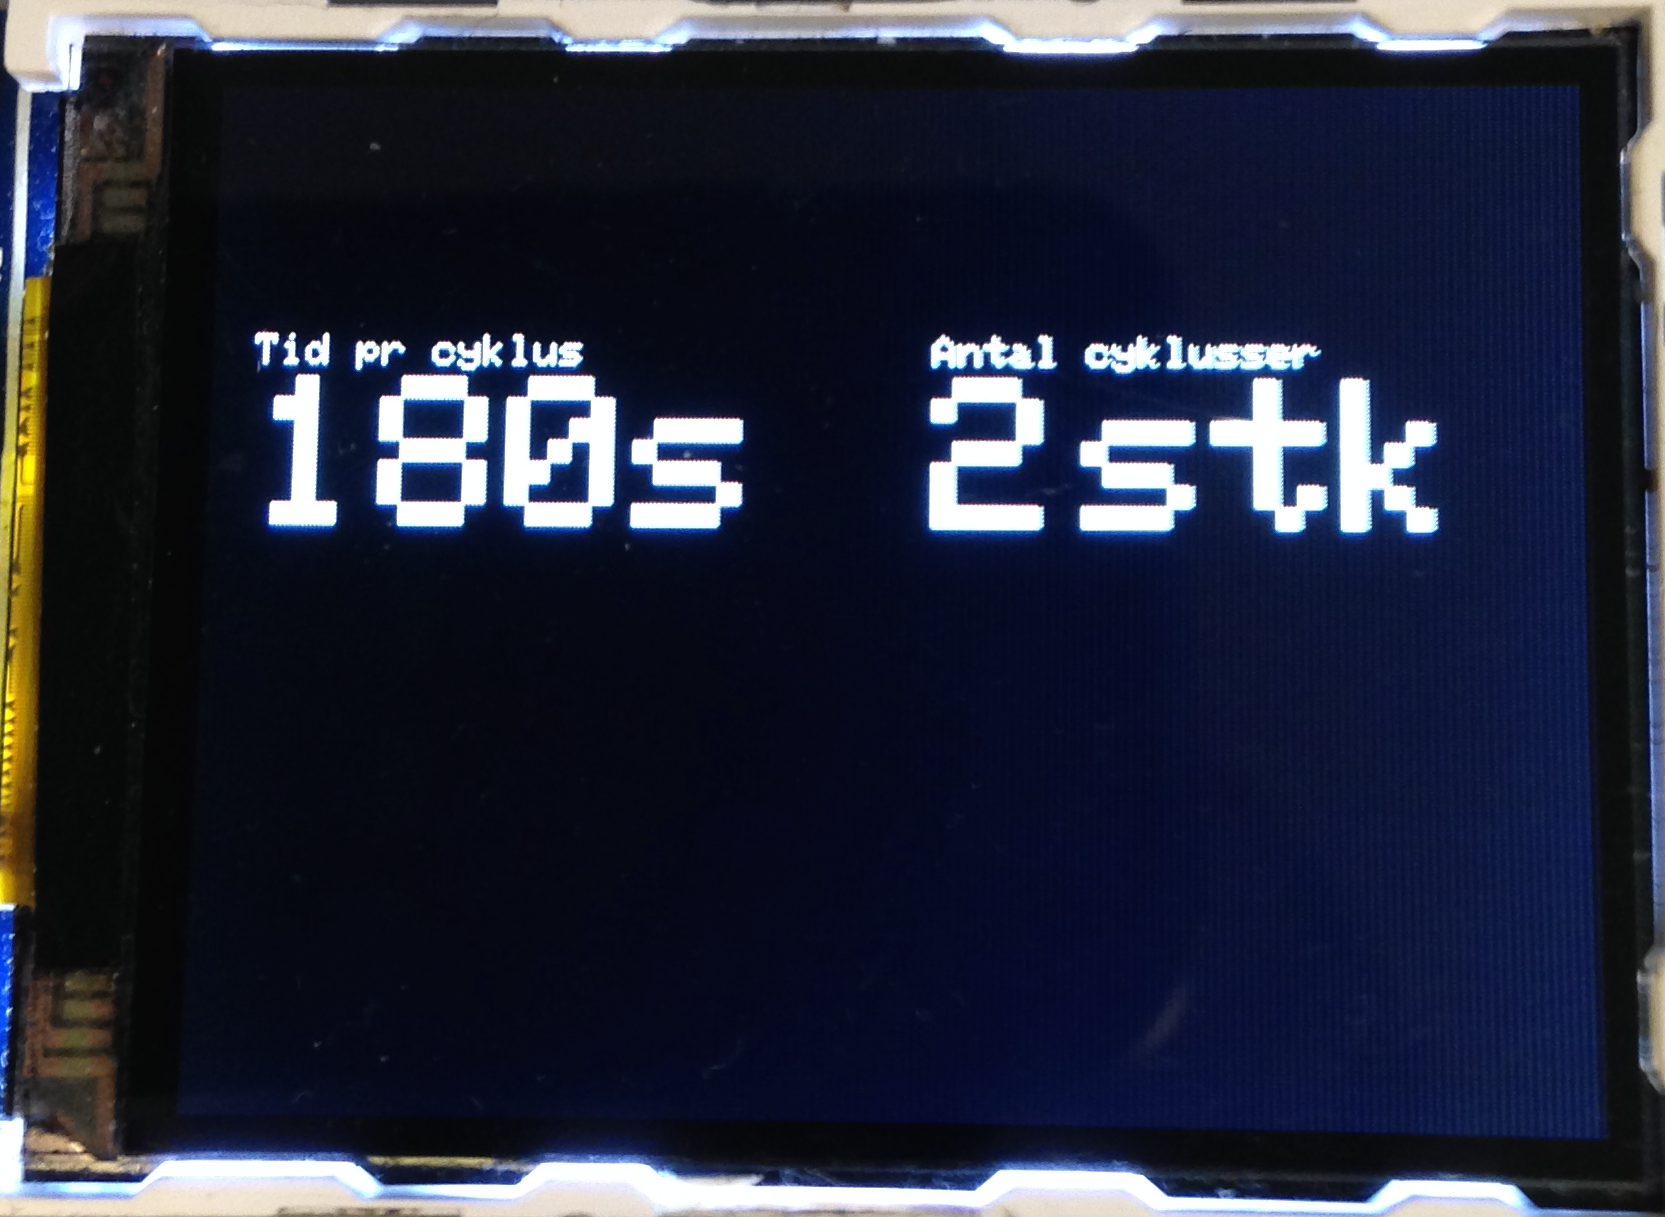
\includegraphics[trim={0 3.3cm 0 1.5cm},clip, width=0.328\textwidth]{billeder/display/setup.png}}
\caption{Billeder over det 3 forskellige programmer \textit{Konditioneringsapparatet} kan udføre. (a) viser en igangværende konditioneringsbehandling, hvor trykket i manchetten ses i midten af billede, blodtrykket lige under. Der ses også patient ID, antal cyklusser og den resterende tid. (b) her vises displayet under okklusionstræning. Manchettrykket visers på skærmen sammen med et stopur. (c) Her vises setup programmet, hvor det er muligt at ændre \textit{tid pr cyklus} og \textit{antal cyklusser} for konditioneringsforløbet vist på (a)}\label{fig:interface}
\end{figure}

\textit{Konditioneringsapparatet} kan som beskrevet før, udføre to andre programmer; hhv. okklusionstræning og setup. Eksempel på brugerfeedback ved de tre forskellige programmer kan ses på figur \ref{fig:interface}. Ved okklusionstræning er kravene til brugerfeedback meget simple, her bliver brugeren informere om det aktuelle tryk i manchetten, som sikre at armen er afklemt tilstrækkeligt under træningssættet. Desuden vises der en tid på skærmen for hvor længe armen har været afklemt. Ved setup programmet består brugerfeedbacken i en blinkende cursor når der skal vælges i mellem \textit{tid pr cyklus} og \textit{antal cyklusser}. Når et af emnerne er valgt, stopper cursoren med at blinke (solid hvid cursor) og brugeren kan ændre i den valgte værdi.

\section{Accepttest}\label{title:accepttest}
Accepttesten blev udført i samarbejde med kunden Rolf Blauenfeldt den 30-11-2015. Accepttesten kan læses i \fixme{ref: accepttest}. Testen forløb uden vejleder Peter Johansen, som ikke kunne være tilstede.

Resultatet ef selve accepttesten er en delvis godkendelse. Alle use cases (UC) blev godkendt med undtagelse af UC 7 (Afbryd) og UC 5 (Sikkerhedskontrold med pulsoximeter). UC 7 opfyldte ikke krav 2.7.3 tilfredsstillende, idet at konditioneringsapparatet ikke med 100\% træfsikkerhed afbrød konditioneringsbehandlingen ved tryk på [Start/Stop]. UC 5 blev aldrig implementeret i konditioneringsapparatet (se afsnit \ref{title:pulsOxi}) og derfor kunne krav 2.5 ikke testes. Læs hvorfor UC 5 ikke blev implementeret under projektafgrænsning i afsnit \ref{title:sikkerhedskontrol}.

De fuldt godkendte use cases var UC 1 (se figur \ref{fig:udsnitAfAccepttest}),2, 3, 4, 6, 8 også kendt som krav 2.1, 2.2, 2.3, 2.4, 2.6, 2.8. Alle ikke funktionelle krav blev godkendt. 

\begin{figure}[H]
	\centering
	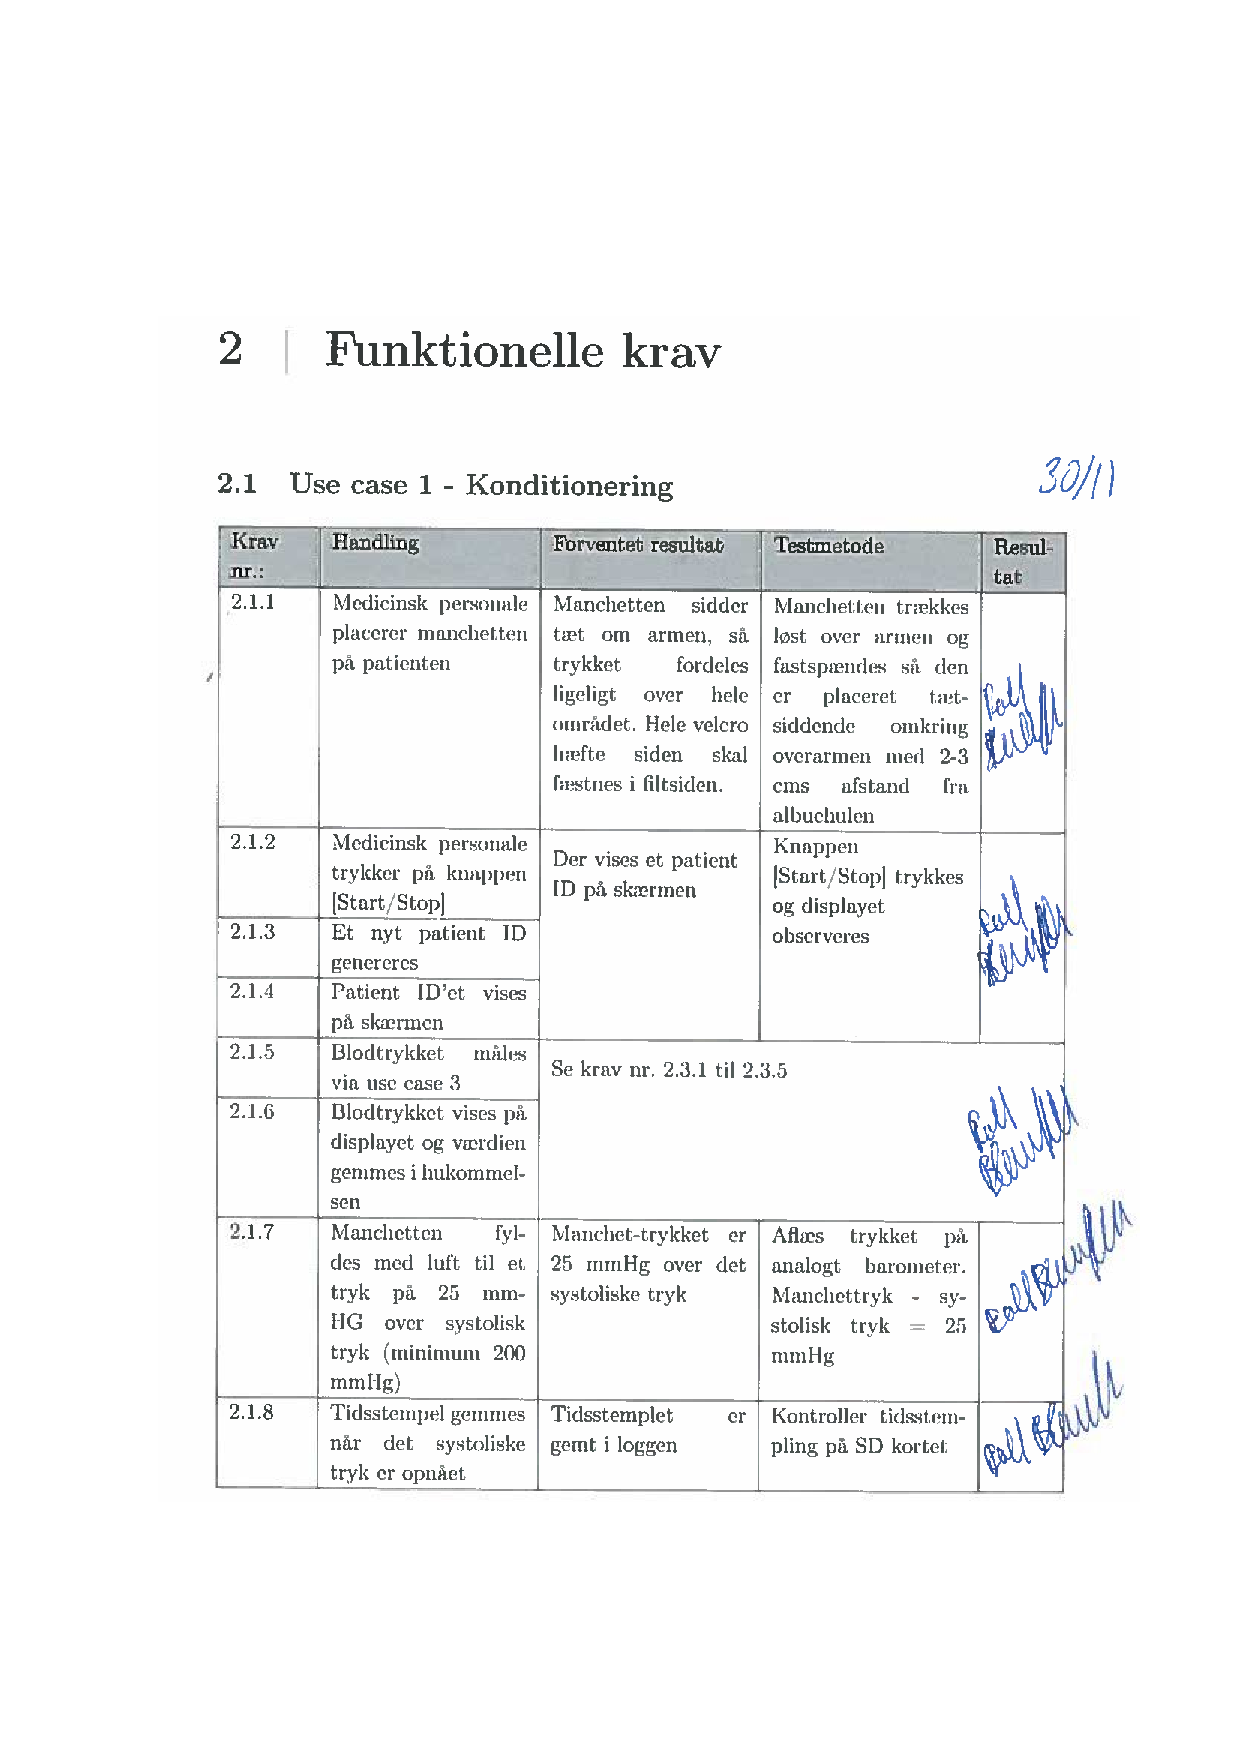
\includegraphics[width=0.6\textwidth]{billeder/udsnitAfAccepttest.pdf}
	\caption{Udsnit af acceptesten foretaget den 30-11-2015. Her ses krav 2.1.1-2.1.8 godkendt. Figuren er scannet af originalen.}\label{fig:udsnitAfAccepttest}
\end{figure}